%******************************************************** -*-LaTeX-*- ******************************
%                                                                                                  *
% v5.0.1.0.4.4.5 Determinante als Natürliche Transformationen.tex                                  *
%                                                                                                  *
% Copyright (C) 2023 Kategory GmbH \& Co. KG (joerg.kunze@kategory.de)                             *
%                                                                                                  *
% v5.0.1.0.4.4.5 Determinante als Natürliche Transformationen is part of kategoryMathematik.       *
%                                                                                                  *
% kategoryMathematik is free software: you can redistribute it and/or modify                       *
% it under the terms of the GNU General Public License as published by                             *
% the Free Software Foundation, either version 3 of the License, or                                *
% (at your option) any later version.                                                              *
%                                                                                                  *
% kategoryMathematik is distributed in the hope that it will be useful,                            *
% but WITHOUT ANY WARRANTY; without even the implied warranty of                                   *
% MERCHANTABILITY or FITNESS FOR A PARTICULAR PURPOSE.  See the                                    *
% GNU General Public License for more details.                                                     *
%                                                                                                  *
% You should have received a copy of the GNU General Public License                                *
% along with this program.  If not, see <http://www.gnu.org/licenses/>.                            *
%                                                                                                  *
%***************************************************************************************************

\documentclass[a4paper]{amsart}
% \documentclass[a4paper]{book}

%-----------------------------------------------------------------------------------------------------*
% package:                                                                                            *
%-----------------------------------------------------------------------------------------------------*
\usepackage{amssymb}
\usepackage{amsfonts}
\usepackage{amsmath}
\usepackage{amsthm}

\usepackage{mathabx}

\usepackage{a4wide} % a little bit smaller margins

\usepackage{graphicx}
\usepackage{hyperref}
\usepackage{algorithmic}
\usepackage{listings}
\usepackage{color}
\usepackage{colortbl}
\usepackage{sidecap}
\usepackage{comment}
\usepackage{tcolorbox}
\usepackage{collect}

\usepackage{upgreek}

% \usepackage{diagrams}

\usepackage[german]{babel}
\usepackage[none]{hyphenat}
\emergencystretch=4em

\usepackage[utf8]{inputenc} % to be able to use äöü as characters in text
\usepackage[T1]{fontenc} % to be able to use äöü in lables
\usepackage{lmodern}     % to avoid pixelation introduced by fontenc

\usepackage{hyperref}

\usepackage{tikz}
\usepackage{tikz-cd}
\usetikzlibrary{babel}

%-----------------------------------------------------------------------------------------------------*
% theorem:                                                                                            *
%-----------------------------------------------------------------------------------------------------*
\theoremstyle{definition}
\newtheorem{theorem}{Theorem}[subsection]

\newcommand{\myTheorem}[1]{%
  \newtheorem{jk#1}[theorem]{#1}
  \newenvironment{#1}[1]{%
    \expandafter\begin{jk#1} \expandafter\label{#1:##1}\textbf{(##1):}
  }{%
    \expandafter\end{jk#1}
  }
}

\myTheorem{Definition}
\myTheorem{Proposition}
\myTheorem{Theorem}
\myTheorem{Example}
\myTheorem{Remark}

\definecollection{jkjkFrage}
\newtheorem{jkFrage}[theorem]{Frage}
\newenvironment{Frage}[1]{%
  \expandafter\begin{jkFrage} \expandafter\label{Frage:#1}\textbf{(#1):}
  \begin{collect}{jkjkFrage}{}{}
    \item \ref{Frage:#1} #1
  \end{collect}
}{%
  \expandafter\end{jkFrage}
}

\newcommand{\myRef}[2]{[#1 \ref{#1:#2}, ``#2'']}

\renewcommand{\proofname}{Beweis}

%-----------------------------------------------------------------------------------------------------*
% operator:                                                                                           *
%-----------------------------------------------------------------------------------------------------*
\DeclareMathOperator{\End}{End}
\DeclareMathOperator{\Ker}{Ker}
\DeclareMathOperator{\Mat}{Mat}
\DeclareMathOperator{\rank}{rank}
\DeclareMathOperator{\ggT}{ggT}
\DeclareMathOperator{\len}{len}
\DeclareMathOperator{\ord}{ord}
\DeclareMathOperator{\kgV}{kgV}
\DeclareMathOperator{\id}{id}
\DeclareMathOperator{\red}{red}
\DeclareMathOperator{\supp}{supp}
\DeclareMathOperator{\Bild}{Bild}
\DeclareMathOperator{\Rang}{Rang}
\DeclareMathOperator{\Det}{Det}
\DeclareMathOperator{\Hom}{Hom}
\DeclareMathOperator{\GL}{GL}

\DeclareMathOperator{\sub}{sub}
\DeclareMathOperator{\blk}{blk}
\DeclareMathOperator{\minimal}{minimal}
\DeclareMathOperator{\maximal}{maximal}

\definecolor{mygreen}{rgb}{0,0.6,0}
\definecolor{mygray}{rgb}{0.5,0.5,0.5}
\definecolor{mymauve}{rgb}{0.58,0,0.82}

\lstset{ %
  backgroundcolor=\color{white},   % choose the background color
  basicstyle=\ttfamily\footnotesize,        % size of fonts used for the code
  breaklines=true,                 % automatic line breaking only at whitespace
  captionpos=b,                    % sets the caption-position to bottom
  commentstyle=\color{mygreen},    % comment style
  escapeinside={\%*}{*)},          % if you want to add LaTeX within your code
  keywordstyle=\color{blue},       % keyword style
  stringstyle=\color{mymauve},     % string literal style
  frame=single
}

\setcounter{MaxMatrixCols}{20}

%******************************************************************************************************
%                                                                                                     *
% definition:                                                                                         *
%                                                                                                     *
%******************************************************************************************************
\newcommand{\R}{\ensuremath{\mathbb{ R }}}
\newcommand{\Q}{\ensuremath{\mathbb{ Q }}}
\newcommand{\Z}{\ensuremath{\mathbb{ Z }}}
\newcommand{\N}{\ensuremath{\mathbb{ N }}}
\newcommand{\C}{\ensuremath{\mathbb{ C }}}
\newcommand{\A}{\ensuremath{\mathbb{ A }}}
\newcommand{\F}{\ensuremath{\mathbb{ F }}}
\newcommand{\K}{\ensuremath{\mathbb{ K }}}
\newcommand{\Pb}{\ensuremath{\mathbb{ P }}}

\newcommand{\M}{\ensuremath{\mathcal{ M }}}
\newcommand{\V}{\ensuremath{\mathcal{ V }}}

\newcommand{\AAA}{\ensuremath{\mathcal{ A }}}
\newcommand{\BB}{\ensuremath{\mathcal{ B }}}
\newcommand{\CC}{\ensuremath{\mathcal{ C }}}
\newcommand{\EE}{\ensuremath{\mathcal{ E }}}
\newcommand{\KK}{\ensuremath{\mathcal{ K }}}
\newcommand{\MM}{\ensuremath{\mathcal{ M }}}
\newcommand{\PP}{\ensuremath{\mathcal{ P }}}
\newcommand{\ZZ}{\ensuremath{\mathcal{ Z }}}

\newcommand{\imporant}[1]{ \textcolor{red}{\textbf{#1}} }

\newcommand{\bb}[1]{\mathbf{#1}}
\newcommand{\balpha}{\boldsymbol{\upalpha}}
\newcommand{\bbeta}{\boldsymbol{\upbeta}}
\newcommand{\bgamma}{\boldsymbol{\upgamma}}
\newcommand{\bdelta}{\boldsymbol{\delta}}
\newcommand{\bmu}{\boldsymbol{\upmu}}

\newcommand{\z}[1]{\Z_{#1}}
\newcommand{\e}[1]{\z{#1}^*}
\newcommand{\q}[1]{(\e{#1})^2}
\newcommand{\m}{\mathcal}

\excludecomment{book}
\excludecomment{example}
\excludecomment{backup}

\begin{document}

%******************************************************************************************************
%                                                                                                     *
\begin{titlepage}
%                                                                                                     *
%******************************************************************************************************
% \vspace*{\fill}
\centering
{\huge
(Höhere Grundlagen) Kategorien\\[1cm]
\textbf{v5.0.1.0.4.4.5 Determinante als Natürliche Transformationen}
}\\[1cm]

\textbf{Kategory GmbH \& Co. KG}\\
Präsentiert von Jörg Kunze\\
Copyright (C) 2023 Kategory GmbH \& Co. KG

\end{titlepage}

%\clearpage
%\setcounter{page}{2}
%
%\tableofcontents

\newpage

%******************************************************************************************************
%                                                                                                     *
\section*{Beschreibung}
%                                                                                                     *
%******************************************************************************************************

%******************************************************************************************************
\subsection*{Inhalt}
%******************************************************************************************************
Die n-dimensionale Determinante ist eine natürliche Transformation.

Zunächst sind die allgemeinen linearen Gruppe und Einheiten-Gruppe zwei Funktoren, was diesen Definitionen jede Beliebigkeit nimmt. Wir haben also zwei Funktoren von der Kategorie der Ringe in die der Gruppen. Anders ausgedrückt: Die Struktur der Ringe untereinander wird zweimal in der Struktur der Gruppen gefunden (als Diagramm).

Darüber hinaus entpuppt sich die Determinante, die jedem Element der allgemeinen linearen Gruppe über einem kommutativen Ring mittels der bekannten Formel ein Element aus dem Ring zuordnet, als Gruppen-Homomorphismus in die Einheiten-Gruppe des Ringes. Das an sich ist schon ein struktureller Erkenntnisgewinn.

Es stellt sich drittens zusätzlich heraus, dass die Determinanten die Komponenten einer natürlichen Transformation vom Allgemeinen-linearen-Gruppen-Funktor zum Einheiten-Gruppen-Funktor sind.

Dies zeigt, wie angemessen die kategorischen Definitionen sind, dass wir sie unter anderem Namen unerkannt oft schon im Bereich unserer Aufmerksamkeit hatten und dass Kategorien-Theorie hilft die Welt zu verstehen.

Es zeigt auch, dass zumindest einige mathematische Strukturen sehr gut zusammen passen und es enthüllt übergreifende Struktur- und Kompatibilitäts-Eigenschaften.

%******************************************************************************************************
\subsection*{Präsentiert}
%******************************************************************************************************
Von Jörg Kunze

%******************************************************************************************************
\subsection*{Voraussetzungen}
%******************************************************************************************************
Axiome der Kategorien, Funktor, natürliche Transformation, Ringe, Determinanten, Einheiten-Gruppe.

%******************************************************************************************************
\subsection*{Text}
%******************************************************************************************************
Der Begleittext als PDF und als LaTeX findet sich unter
{\tiny
   \url{https://github.com/kategory/kategoryMathematik/tree/main/v5%20H%C3%B6here%20Grundlagen/v5.0.1%20Kategorien/v5.0.1.0.4.4.5%20Determinante%20als%20Nat%C3%BCrliche%20Transformationen}
}

%******************************************************************************************************
\subsection*{Meine Videos}
%******************************************************************************************************
Siehe auch in den folgenden Videos:\\
v5.0.1.0.3 (Höher) Kategorien - Funktoren\\
\url{https://youtu.be/Ojf5LQGeyOU}\\
v5.0.1.0.4 (Höher) Kategorien - Natürliche Transformationen\\
\url{https://youtu.be/IN7Qa-SwlD0}\\

%******************************************************************************************************
\subsection*{Quellen}
%******************************************************************************************************
Siehe auch in den folgenden Seiten:\\
\url{https://de.wikipedia.org/wiki/Nat%C3%BCrliche_Transformation}\\
\url{https://ncatlab.org/nlab/show/natural+transformation}\\
\url{https://de.wikipedia.org/wiki/Funktor_(Mathematik)}\\
\url{https://de.wikipedia.org/wiki/Ring_(Algebra)}\\
\url{https://de.wikipedia.org/wiki/Determinante}\\
\url{https://de.wikipedia.org/wiki/Determinante#Determinantenproduktsatz}\\
\url{https://de.wikipedia.org/wiki/Einheitengruppe}

%******************************************************************************************************
\subsection*{Buch}
%******************************************************************************************************
Grundlage ist folgendes Buch:\\
"`Categories for the Working Mathematician"'\\
Saunders Mac Lane\\
1998 | 2nd ed. 1978\\
Springer-Verlag New York Inc.\\
978-0-387-98403-2 (ISBN)\\
{\tiny
   \url{https://www.amazon.de/Categories-Working-Mathematician-Graduate-Mathematics/dp/0387984038}}\\

Gut für die kategorische Sichtweise ist:\\
"`Topology, A Categorical Approach"'\\
Tai-Danae Bradley\\
2020 MIT Press\\
978-0-262-53935-7 (ISBN)\\ 
{\tiny
\url{https://www.lehmanns.de/shop/mathematik-informatik/52489766-9780262539357-topology}}\\

Einige gut Erklärungen finden sich auch in den Einführenden Kapitel von:\\
"`An Introduction to Homological Algebra"'\\
Joseph J. Rotman\\
2009 Springer-Verlag New York Inc.\\
978-0-387-24527-0 (ISBN)\\ 
{\tiny \url{https://www.lehmanns.de/shop/mathematik-informatik/6439666-9780387245270-an-introduction-to-homological-algebra}}\\

Etwas weniger umfangreich und weniger tiefgehend aber gut motivierend ist:
"`Category Theory"'\\
Steve Awodey\\
2010 Oxford University Press\\
978-0-19-923718-0 (ISBN)\\
{\tiny\url{https://www.lehmanns.de/shop/mathematik-informatik/9478288-9780199237180-category-theory}}\\

Mit noch weniger Mathematik und die Konzepte motivierend ist:
"`Conceptual Mathematics: a First Introduction to Categories"'\\
F. William Lawvere, Stephen H. Schanuel\\
2009 Cambridge University Press\\
978-0-521-71916-2 (ISBN)\\
{\tiny\url{https://www.lehmanns.de/shop/mathematik-informatik/8643555-9780521719162-conceptual-mathematics}}

%******************************************************************************************************
\subsection*{Lizenz}
%******************************************************************************************************
Dieser Text und das Video sind freie Software. Sie können es unter den Bedingungen der 
GNU General Public License, wie von der Free Software Foundation veröffentlicht, weitergeben 
und/oder modifizieren, entweder gemäß Version 3 der Lizenz oder (nach Ihrer Option) jeder späteren Version.

Die Veröffentlichung von Text und Video erfolgt in der Hoffnung, dass es Ihnen von Nutzen sein wird, 
aber OHNE IRGENDEINE GARANTIE, sogar ohne die implizite Garantie der MARKTREIFE oder der 
VERWENDBARKEIT FÜR EINEN BESTIMMTEN ZWECK. Details finden Sie in der GNU General Public License.

Sie sollten ein Exemplar der GNU General Public License zusammen mit diesem Text erhalten haben 
(zu finden im selben Git-Projekt). 
Falls nicht, siehe \url{http://www.gnu.org/licenses/}.

\subsection*{Das Video}
%******************************************************************************************************
Das Video hierzu ist zu finden unter 
{\tiny
   \url{https://youtu.be/kgTqHLaolMc}
}

%******************************************************************************************************
%                                                                                                     *
\section{Determinante ist natürliche Transformation}
%                                                                                                     *
%******************************************************************************************************
Allgemein seine im folgenden $R, S$ kommutative Ringe mit $1$.

%******************************************************************************************************
\subsection{Allgemeine lineare Gruppe ist Funktor}
%******************************************************************************************************
Die allgemeine lineare Gruppe ist die Zuordnung
\begin{align}
   \GL_n \colon \text{\textbf{Ring}} \to \text{\textbf{Gruppe}}\\
   R \mapsto \GL_n(R),
\end{align}
Wobei $\GL_n(R)$ die Gruppe der invertierbaren $n \times n$-Matrizen mit Koeffizienten in $R$ ist.
Damit das ein Funktor sein kann, müssen wir die Abbildung auf Morphismen erweitern und zeigen, dass die Axiome für Funktoren erfüllt sind.

Sei $f \colon R \to S$ ein Ring-Homomorphismus. Dann definieren wir eine Abbildung 
\begin{align}
   \GL_n(f) \colon \GL_n( R ) \to \GL_n( S )\\
   (a_{ij}) \mapsto (f( a_{ij} )).
\end{align}
Da die Matrix-Multiplikation auf die Grundrechenarten zurückzuführen sind, und diese Grundrechenarten mit $f$ vertauschen, ist der Nachweis, dass es sich bei $\GL_n(f)$ um einen Gruppen-Homomorphismus handelt, leicht.

Die Axiome eines Funktors
\begin{align}
   \GL_n(\id_R) &= \id_{\GL_n( R )}\\
   \GL_n(f \circ g) &= \GL_n(f) \circ \GL_n(g)
\end{align}
sind noch einfacher nachzuweisen.

%******************************************************************************************************
\subsection{Einheiten-Gruppe ist Funktor}
%******************************************************************************************************
Wir definieren die Einheiten-Gruppe als
\begin{equation}
   R^* := \{r \in R \mid \exists r' \in R \colon rr' = r'r = 1 \},
\end{equation}
also als die Menge der multiplikativ invertierbaren Elemente von $R$. Dabei vergessen wir noch die Addition und erhalten eine Gruppe mit der Multiplikation als Verknüpfung. Wir definieren weiter $f^*(r) :=  f(r)$ und benutzen die Tatsache, dass das Bild einer Einheit eine Einheit ist, um die Funktor-Axiome für $\_^*$ nachzuweisen.

%******************************************************************************************************
\subsection{Determinante ist Gruppen-Homomorphismus}
%******************************************************************************************************
Die Aussage, dass Abbildung
\begin{align}
   \Det_n^R \colon &\GL_n(R) \to R^*\\
                   &M \mapsto \Det_n^R 
\end{align}
ist ein Gruppenhomomorphismus ist, ist die selbe wie der Determinantenproduktsatz:
\begin{equation}
   \Det_n^R(MN) = \Det_n^R(M) \Det_n^R(N).
\end{equation} 

%******************************************************************************************************
\subsection{Determinante ist natürliche Transformation}
%******************************************************************************************************
Genauer: für jedes $n$ ist die $n$-dimensionale Determinante $\Det_n$ eine natürliche Transformation mit den Komponenten $\Det_n^R$ mit $R \in \text{\textbf{Ring}}$.

Wir wissen schon:
\begin{itemize}
   \item Allgemeine lineare Gruppe ist Funktor von \textbf{Ring} nach \textbf{Gruppe},
   \item Einheiten-Gruppe ist Funktor von \textbf{Ring} nach \textbf{Gruppe},
   \item Determinante ist Gruppen-Homomorphismus.
\end{itemize}
Um nachzuweisen, dass die Determinante eine natürliche Transformation genügt es somit, die Vertauschbarkeit mit den beiden involvierten Funktoren nachzuweisen.

Sei dazu $f \colon R \to S$ ein Ring-Homomorphismus. Es muss also die Kommutativität des folgenden Diagramms gezeigt werden:
\begin{equation}\label{kommutativ}
   \begin{tikzcd}
      \mathcal \GL_n(R) \arrow[r, "\Det_n^R"] \arrow[d, "\GL_n(f)"]
      &R^* \arrow[d, "f^*"]\\
      \GL_n(S) \arrow[r, "\Det_n^S"]  
      & S^*\\
   \end{tikzcd}
\end{equation}
\begin{proof}
   Sei dazu $(a_{ij}) \in \GL_n(R)$. Wir bezeichnen mit $D( X_1, \cdots, X_n)$ das Polynom in $n$ Variablen, welches die Determinante als Funktion der Koeffizienten ausrechnet. Dann gilt:
   \begin{align}
      &&&\Det_n^S( \GL_n(f) )( (a_{ij}) )\\
      &=&&\Det_n^S( ( f(a_{ij}) ) )       &&\text{ $\GL_n(f)$ ist Anwendung von $f$ auf Koeffizienten}\\
      &=&&D( ( f(a_{ij}) ) )              &&\text{ Determinante als Polynom ausgerechnet}\\
      &=&&f( D( (a_{ij}) ) )            &&\text{ da $f$ Ring-Homomorphismus}\\
      &=&&f^*D( ( a_{ij}) ) )            &&\text{ da $f^*$ die Einschränkung von $f$ auf die Einheiten ist}\\
      &=&&f^*( \Det_n^R( (a_{ij}) ) )     &&\text{ Determinante als Polynom ausgerechnet}
   \end{align}
\end{proof}

Mit 
\begin{equation}
   D( (a_{ij}) )={\begin{vmatrix}a_{1,1}\ldots a_{1,n}\\\vdots \qquad \vdots \\a_{n,1}\ldots a_{n,n}\end{vmatrix}}=\sum _{\sigma \in S_{n}}\operatorname {sgn}(\sigma )a_{1,\sigma _{1}}\cdots a_{n,\sigma _{n}}
\end{equation}

%******************************************************************************************************
\subsection{Graphische Veranschaulichung}
%******************************************************************************************************
\begin{figure}[h]
   \centering
   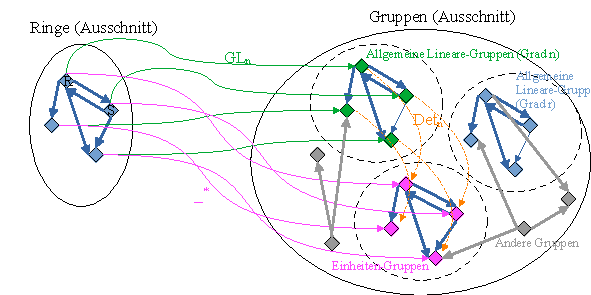
\includegraphics[width=\textwidth]{v5.0.1.0.4.4.5 Determinante als Natürliche Transformationen Bild.pdf}
\end{figure}

Wir finden den Graph der Kategorie der Ringe mehrmals als Diagramme im Graph der Kategorie der Gruppen. Die natürliche Transformation überführt diese ähnlichen Diagramme ineinander, ud das kompatible zu den Bildern der Homomorphismen.

%******************************************************************************************************
\subsection{Liste der Tatsachen, die in der Aussage "`Det ist Nat"' enthalten sind}
%******************************************************************************************************
Wieder ein Beispiel dafür, wie viel in einem Satz wie "`Determinante ist natürliche Transformation"' enthalten ist:
\begin{itemize}
   \item Lineare Gruppe ist Funktor: kann auf Morphismen erweitert werden und es gelten die Funktoraxiome
   \item Einheitengruppe ist Funktor: kann auf Morphismen erweitert werden und es gelten die Funktoraxiome
   \item Determinate ist Gruppenhomomorphismus
\end{itemize}

In den Satz "`Determinante ist natürliche Transformation"' fließen folgende Tatsachen ein: 
\begin{itemize}
   \item Bild einer Einheit ist Einheit
   \item Determinantenproduktsatz
   \item Determinante ist als Polynom mit Ring-Homomorphismen verträglich
   \item Determinante einer invertierbaren Matrix ist nicht null
\end{itemize}

%******************************************************************************************************
%                                                                                                     *
\section{TODO}
%                                                                                                     *
%******************************************************************************************************
\begin{backup}
Noch zu erledigen sind
\begin{itemize}
   \item leer
\end{itemize}
\end{backup}

\begin{backup}
    (Zur Zeit nicht benötigter Inhalt)
\end{backup}

%******************************************************************************************************
%                                                                                                     *
\begin{thebibliography}{9}
%                                                                                                     *
%******************************************************************************************************
   \bibitem[Awodey2010]{Awodey}
      Steve Awode, \emph{Category Theory},
      2010 Oxford University Press, 978-0-19-923718-0 (ISBN)

   \bibitem[Bradley2020]{Bradley}
      Tai-Danae Bradley, \emph{Topology, A Categorical Approach},
      2020 MIT Press, 978-0-262-53935-7 (ISBN)

   \bibitem[LawvereSchanuel2009]{Lawvere}
      F. William Lawvere, Stephen H. Schanuel, \emph{Conceptual Mathematics: a First Introduction to Categories},
      2009 Cambridge University Press, 978-0-521-71916-2 (ISBN)

   \bibitem[MacLane1978]{MacLane}
      Saunders Mac Lane, \emph{Categories for the Working Mathematician},
      Springer-Verlag New York Inc., 978-0-387-98403-2 (ISBN)

   \bibitem[Rotman2009]{Rotman}
   	Joseph J. Rotman, \emph{An Introduction to Homological Algebra},
   	2009 Springer-Verlag New York Inc., 978-0-387-24527-0 (ISBN)
      
\end{thebibliography}

%******************************************************************************************************
%                                                                                                     *
\begin{large}
    \centerline{\textsc{Symbolverzeichnis}}
\end{large}
%                                                                                                     *
%******************************************************************************************************
\bigskip

\renewcommand*{\arraystretch}{1}

\begin{tabular}{ll}
    $A, B, C, \cdots, X, Y, Z$          & Objekte\\
    $\mathcal F,\mathcal G$             & Funktoren\\
    $f, g, h, r, s, \cdots$             & Homomorphismen\\
    $\mathcal C, \mathcal D, \mathcal E, \cdots$ & Kategorien\\
    \textbf{Set}                        & Die Kategorie der Mengen\\
    $\Hom( X, Y)$                       & Die Menge der Homomorphismen von $X$ nach $Y$\\
    $\alpha, \beta, \cdots$             & natürliche Transformationen\\
    $\mathcal C ^{\text{op}}$           & Duale Kategorie\\
    \textbf{Ring} nach \textbf{Gruppe}  & Kategorie der Ringe und der Gruppen\\
    $\GL_n(R)$                          & Allgemeine lineare Gruppe über dem Ring $R$\\
    $R^*$                               & Einheitengruppe des Rings $R$\\
    $\Det_n^R$                          & $n$-dimensionale Determinante für Matrizen mit Koeffizienten in $R$. 
    
\end{tabular}

\end{document}
